\section{Project Introduction}
\subsection{Overview}
This report documents the design, implementation, and evaluation of AL-QNN, a variational quantum classifier whose circuit depth is adjusted online by a reinforcement-learning agent in order to keep the model trainable in the presence of barren plateaus. Section~2 describes the project management plan. Section~3 reviews the state of the art in quantum machine learning and barren-plateau mitigation. Section~4 details the reinforcement-learning methodology. Section~5 presents the system design and implementation. Section~6 reports and discusses the results across several backends and cost regimes, with particular attention to when adaptive scheduling helps and when it does not. Section~7 concludes and outlines future work.

\subsection{Background and Motivation}
Variational quantum algorithms are among the most promising candidates for demonstrating practical value on today's Noisy Intermediate-Scale Quantum (NISQ) hardware. They combine a parameterized quantum circuit with a classical optimizer, so that the quantum device only has to execute shallow circuits while the heavy optimization runs classically. However, a fundamental obstacle stands in the way: the barren-plateau phenomenon. As the number of qubits grows, the variance of the cost-function gradient vanishes exponentially, so the optimizer receives essentially no signal and training stalls.

A natural but naive response is to fix the circuit depth in advance. This fails in both directions: a circuit that is too shallow cannot express the target function (underfitting), while a circuit that is too deep sinks deeper into the barren-plateau region and becomes untrainable. Choosing the right depth by hand for every dataset and qubit count is impractical. This project asks whether a reinforcement-learning agent can instead schedule the depth online -- adding capacity when gradients are healthy and pruning it when they are not -- using live telemetry from the circuit itself.

This question sits at the intersection of two active research programs. On the quantum side, the community has largely treated barren plateaus as a property to be measured and, where possible, avoided by construction -- through initialization strategies, restricted ansatz families, or problem-inspired circuit designs (Section~3). Comparatively little work treats the plateau as something to be actively managed at training time by an agent that observes it directly. On the machine-learning side, reinforcement learning has repeatedly proven effective at exactly this kind of online resource-allocation problem -- deciding, step by step, how much capacity or compute to commit to a task based on live feedback -- in domains from neural architecture search to robotics. AL-QNN sits at the overlap: it applies an RL formulation, otherwise unremarkable, to a resource-allocation decision (circuit depth) that is unremarkable in machine learning generally but has a genuinely quantum-specific failure mode (the barren plateau) driving it.

A further practical motivation is that near-term quantum devices are themselves resource-constrained: circuit depth is not a free parameter even ignoring trainability, because deeper circuits accumulate more gate error and take longer to execute on real hardware. A scheduler that commits to the shallowest depth sufficient for a given dataset and cost regime is therefore not only a trainability aid but also, in principle, a resource-efficiency mechanism -- a secondary benefit that this project does not evaluate directly (Section~1.6) but that motivates why depth, specifically, rather than some other circuit hyperparameter, was chosen as the control variable.

\subsection{Project Objective}
The high-level objective is to build and evaluate an RL agent that adaptively schedules the depth of a hardware-efficient variational circuit so as to maintain trainable gradients while achieving competitive classification performance. Concretely, the project aims to:

\begin{itemize}
\item Characterize the barren-plateau regime empirically as a function of qubit count and circuit depth on real datasets.
\item Design a Markov Decision Process in which an agent observes circuit telemetry and chooses to add, prune, or hold layers.
\item Train PPO and DQN agents efficiently using a fast classical surrogate, then deploy the learned policy on a PennyLane statevector simulator.
\item Evaluate the scheduler against static baselines (a hand-tuned rule and a greedy heuristic) across several regimes, and honestly characterize the conditions under which adaptive scheduling provides an advantage.
\end{itemize}

\subsection{Problem Statement}
Formally, training a variational quantum circuit means minimizing a cost function $C(\theta)$ over the circuit parameters $\theta$. Under a global cost and a sufficiently expressive ansatz, the gradient variance $\mathrm{Var}[\partial C/\partial\theta]$ decays as $O(2^{-n})$ in the qubit count $n$ \citep{mcclean2018barren}; this is the barren plateau. In this regime the optimizer's updates are dominated by shot noise and the loss does not decrease. The severity also depends on the cost definition: a local cost weakens the plateau but introduces a dependence on circuit depth \citep{cerezo2021cost}, so depth becomes a genuine control variable rather than a free parameter.

\begin{figure}[htbp]
\centering
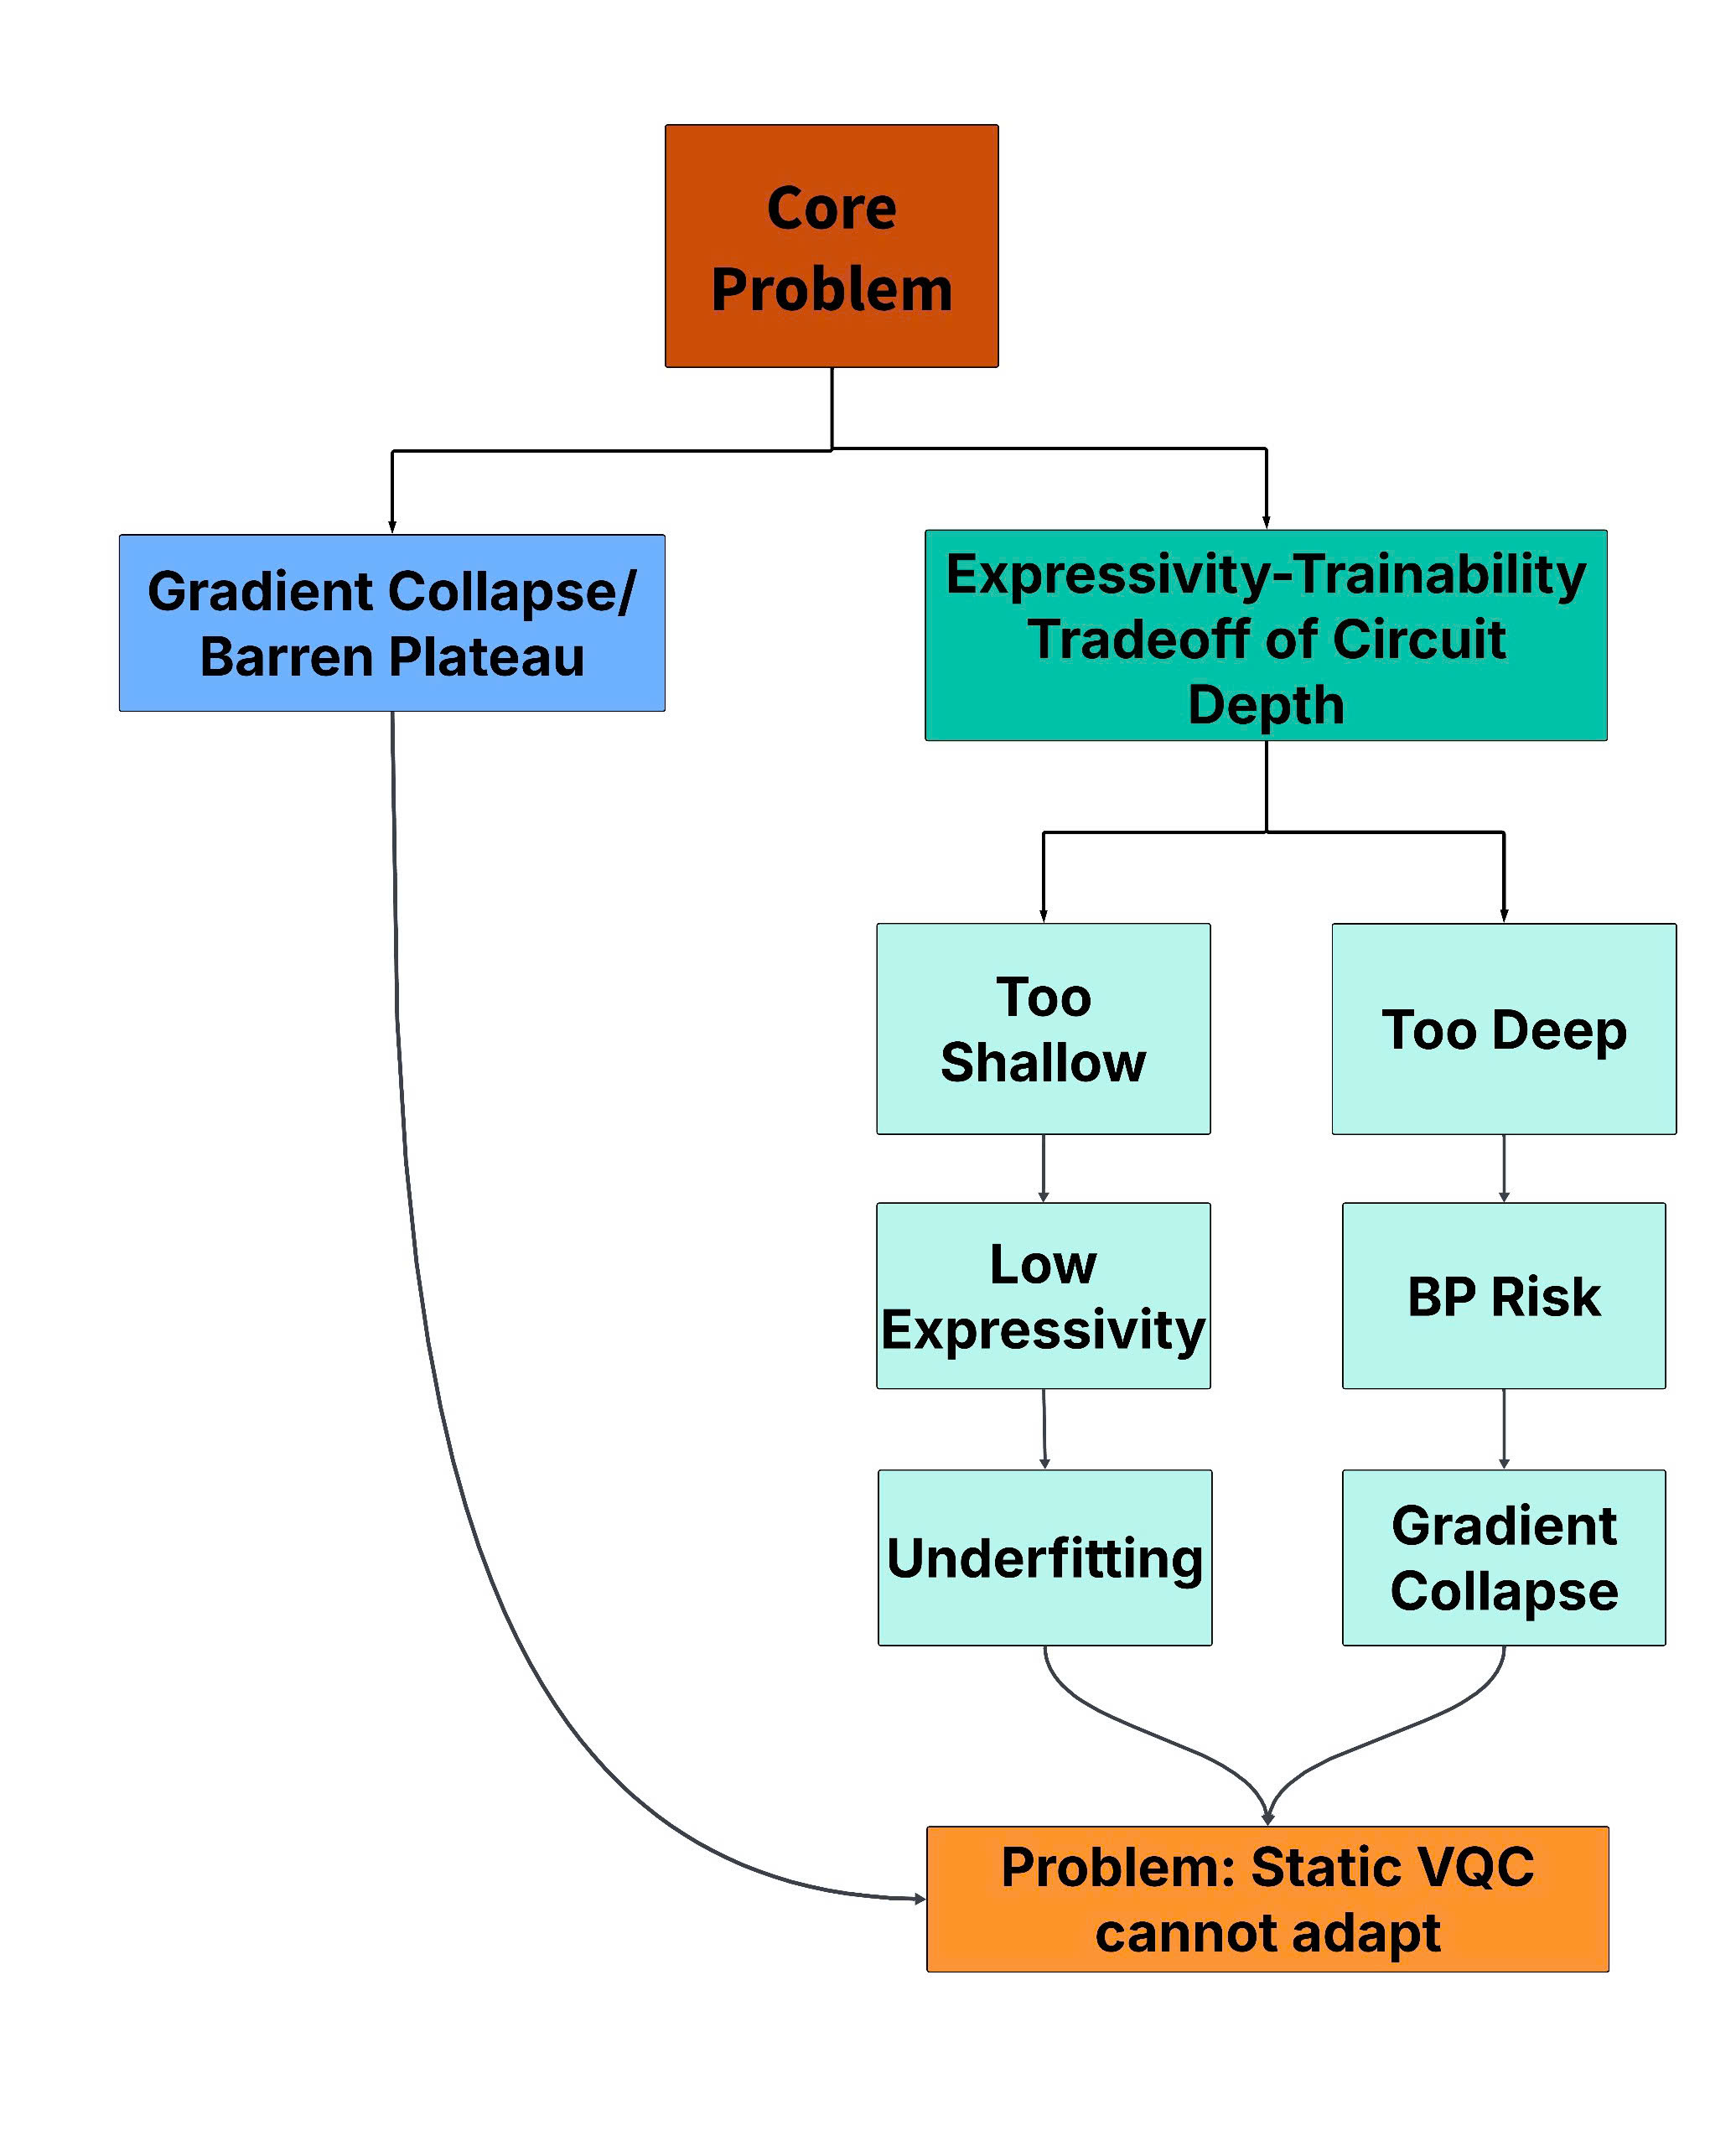
\includegraphics[width=0.75\textwidth]{figure/fig_problem_framing.jpg}
\caption{Problem framing. A fixed circuit depth fails in both directions: too shallow gives low expressivity and underfitting; too deep raises barren-plateau risk and gradient collapse. Both paths, together with the separate qubit-count-driven barren-plateau mechanism, converge on the same obstacle -- a static VQC cannot adapt to what the data and the current training state actually require.}
\label{fig:problem_framing}
\end{figure}

The engineering problem is therefore twofold. First, the depth of the circuit must be chosen adaptively, because the correct depth depends on the dataset, the qubit count, and the cost type, none of which are known a priori. Second, any adaptation must be driven by information that is actually observable during training -- gradient magnitudes, loss dynamics, and near-zero-gradient ratios -- rather than by an oracle. The project addresses both by casting depth scheduling as a reinforcement-learning problem over circuit telemetry.

A third, more subtle requirement follows from the first two: because the correct depth is regime-dependent rather than universal, any claim that a given scheduler is ``better'' is only meaningful relative to a specific dataset, qubit count, and cost type. A scheduler that wins in one regime may lose in another, and an evaluation methodology that reports results from only one regime risks presenting a partial, misleadingly general picture. This is why Section~6 deliberately reports results across several regimes (one real deployment and a synthetic comparison isolating cost type, all at the qubit counts validated on available hardware) rather than a single headline number: the project's empirical contribution is as much about characterizing the boundary of where adaptive scheduling helps as it is about the scheduler itself. Section~6.1 additionally reports three supplementary single-seed real deployments on other datasets (German Credit, Parkinson's, Pima); these sit outside the core evaluation design and are not weighted as evenly as the core regimes, but they were already available from the project's data-preparation work and are reported for completeness rather than left undocumented.

\subsection{Significance of the Project}
The theoretical contribution is a principled, telemetry-driven formulation of circuit-depth scheduling as an MDP, together with an honest empirical characterization of the regime in which reinforcement learning improves on simple static baselines. Rather than claiming universal superiority, the project identifies the specific conditions -- principally a local cost, where the plateau is depth-dependent rather than fixed -- under which adaptive scheduling separates from static schedulers. This nuanced result is itself a useful finding for practitioners.

The practical contribution is a reusable two-simulator architecture that makes RL training tractable for quantum circuits: a fast classical surrogate for the millions of environment steps required by RL, and a PennyLane statevector backend for faithful deployment and evaluation. The same pipeline is demonstrated on a real deployment (Heart Disease) and on a synthetic comparison isolating cost type.

\subsection{Scope and Limitations}
\textbf{Scope.} The project covers binary classification with hardware-efficient variational circuits, at up to 8 qubits on real datasets; evaluation runs on a statevector simulator (PennyLane) and on a calibrated classical surrogate (Section~4.7.1). The 8-qubit ceiling is a hardware limitation, not a design choice: PennyLane's statevector simulation and the RL deployment loop built on top of it become impractically slow and memory-hungry on the team's available machines beyond this range, so larger qubit counts were not pursued for the results reported here. The reinforcement-learning agent schedules circuit depth (add/prune/hold) and entanglement adjustments, trained with PPO and DQN. Preprocessing, barren-plateau measurement, deployment, and a demonstration interface are all included.

\textbf{Limitations.} Results are obtained on a noiseless statevector simulator, not on physical NISQ hardware; hardware noise is out of scope. The 8-qubit ceiling (above) means the barren-plateau scaling and the primary AI4I benchmark, both of which need a wider qubit range to show a strong effect, are correspondingly modest; AI4I was used with three seeds during development to characterize seed variance, and the scheduler-comparison tables presented in Section~6 are single-seed across datasets, backends, and cost regimes, and are labelled as exploratory.

